%Anexo con imágenes analizadas con algoritmo de procesamiento homomórfico

\begin{figure}[h!]
    \includegraphics[width=0.5\textwidth]{Imagenes/Homomorfico/Paranai1eq.png}
     \hfill
     \caption{Imagen aérea (satelital) de una porción de selva nativa y terrenos cultivados junto al arroyo Paranay }
    %\label{Paranay1}
\end{figure}

\begin{figure}
    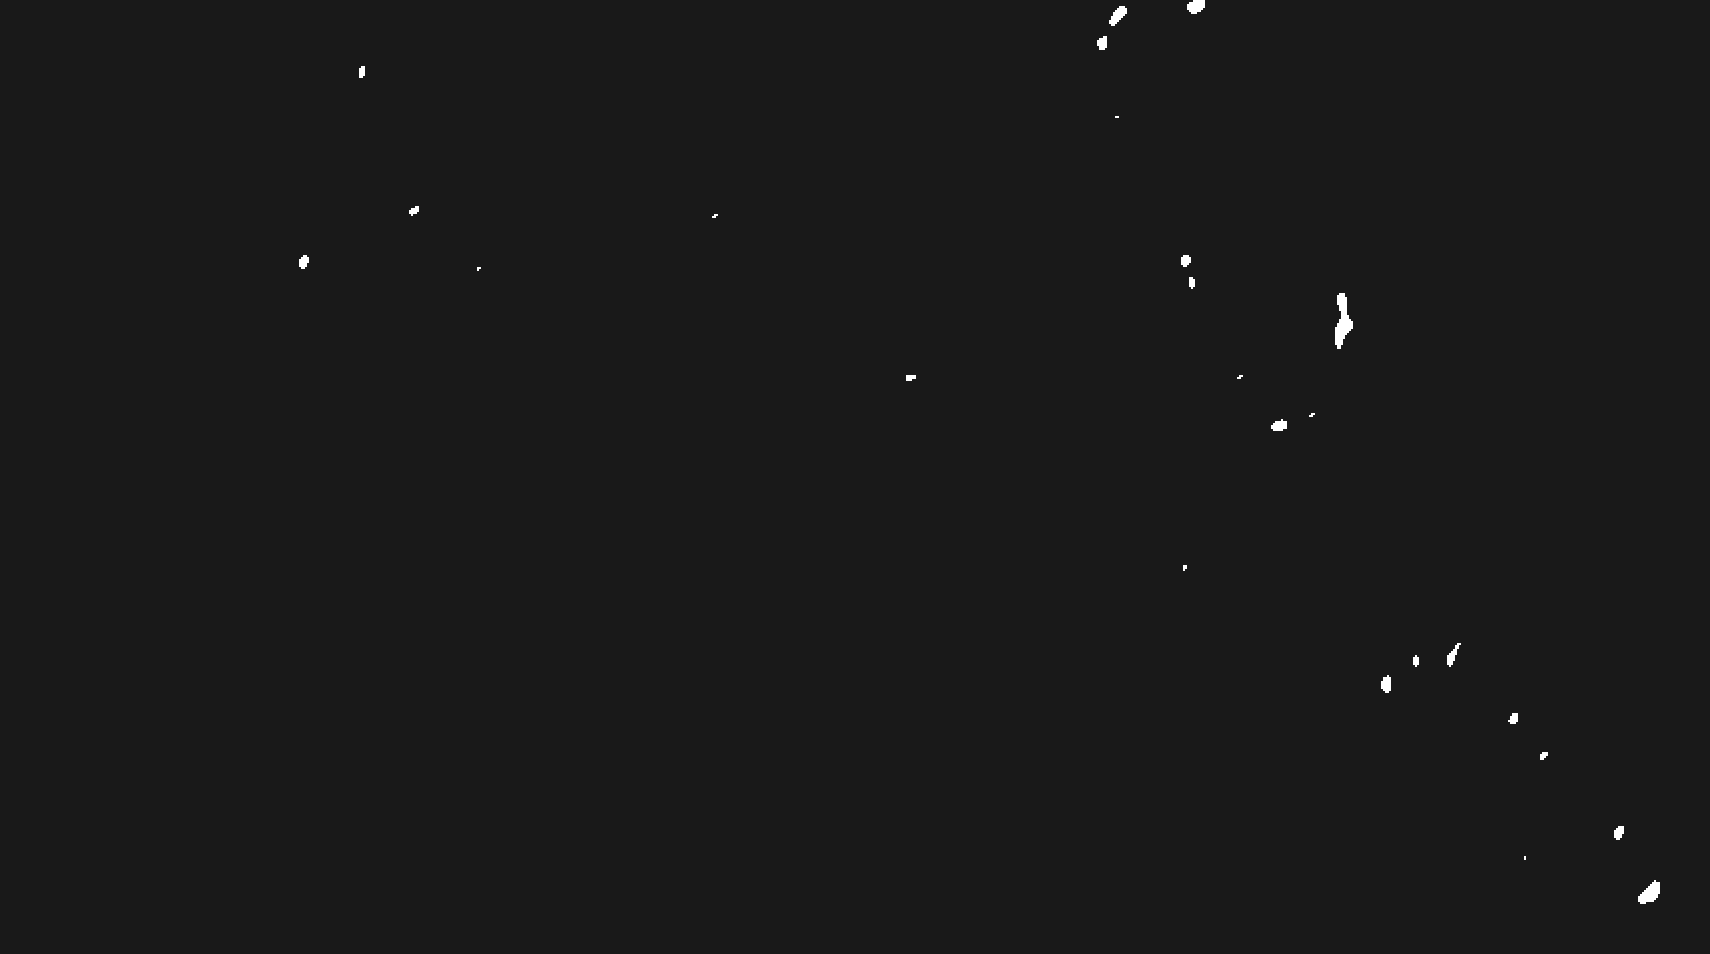
\includegraphics[width=.3\textwidth]{Imagenes/Homomorfico/Paranai1_bin.png}\hfill
    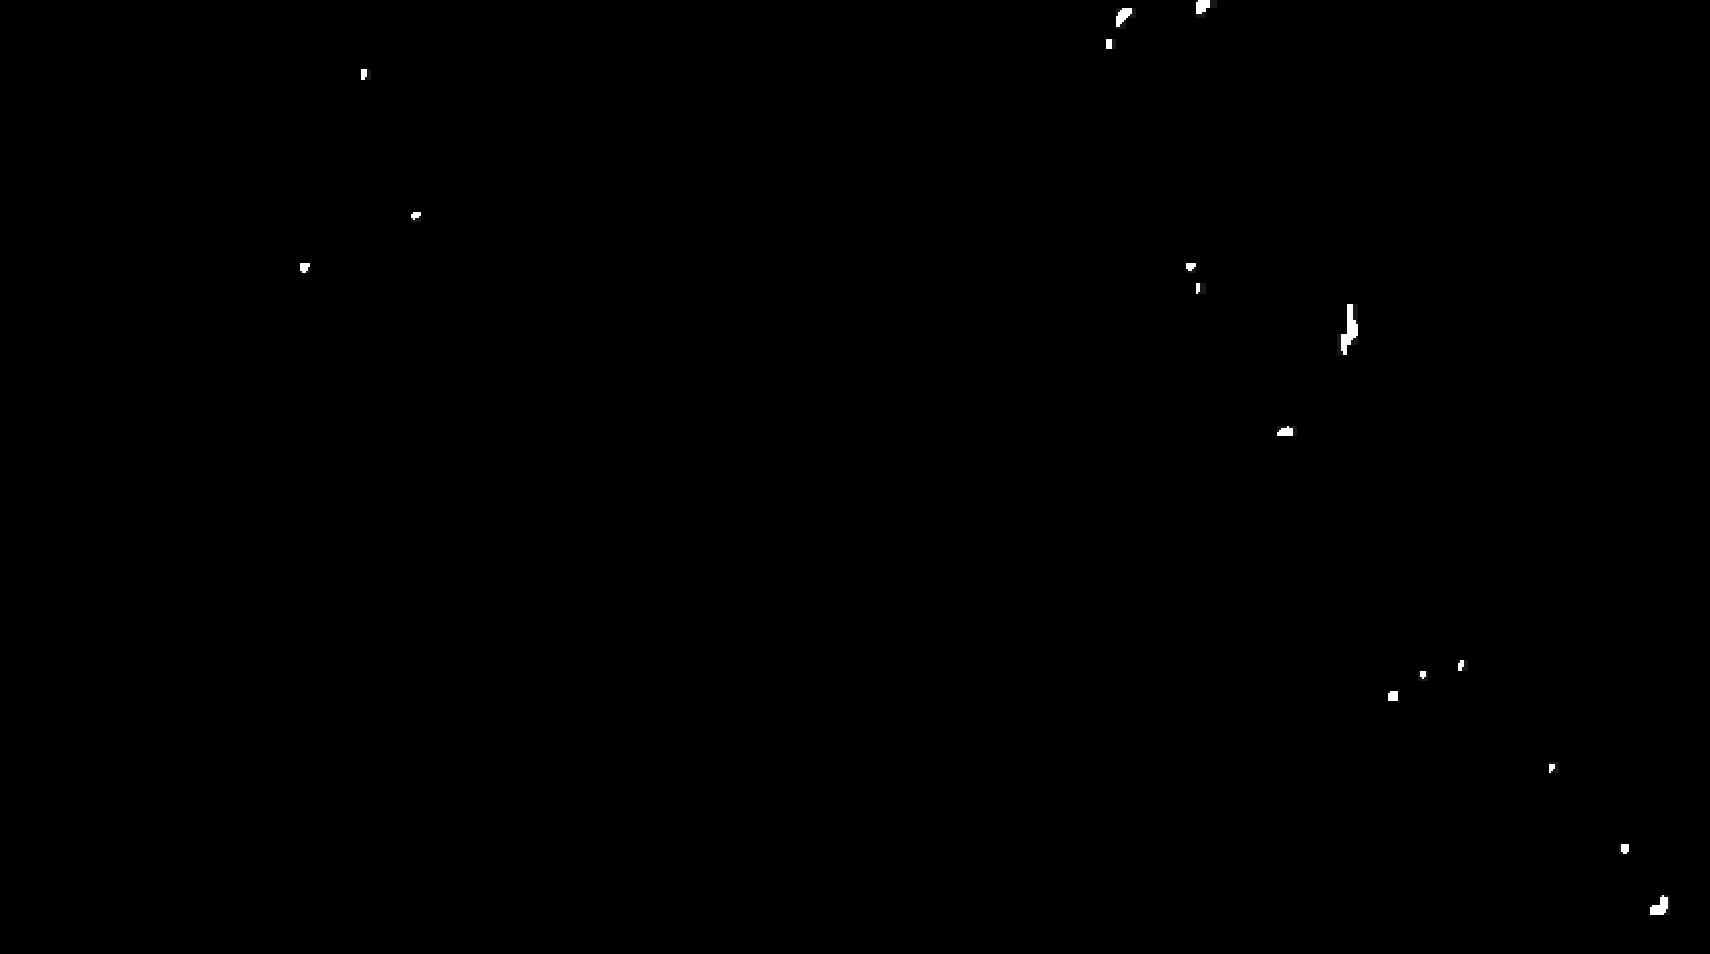
\includegraphics[width=.3\textwidth]{Imagenes/Homomorfico/Paranai1_masked_10.png}\hfill
    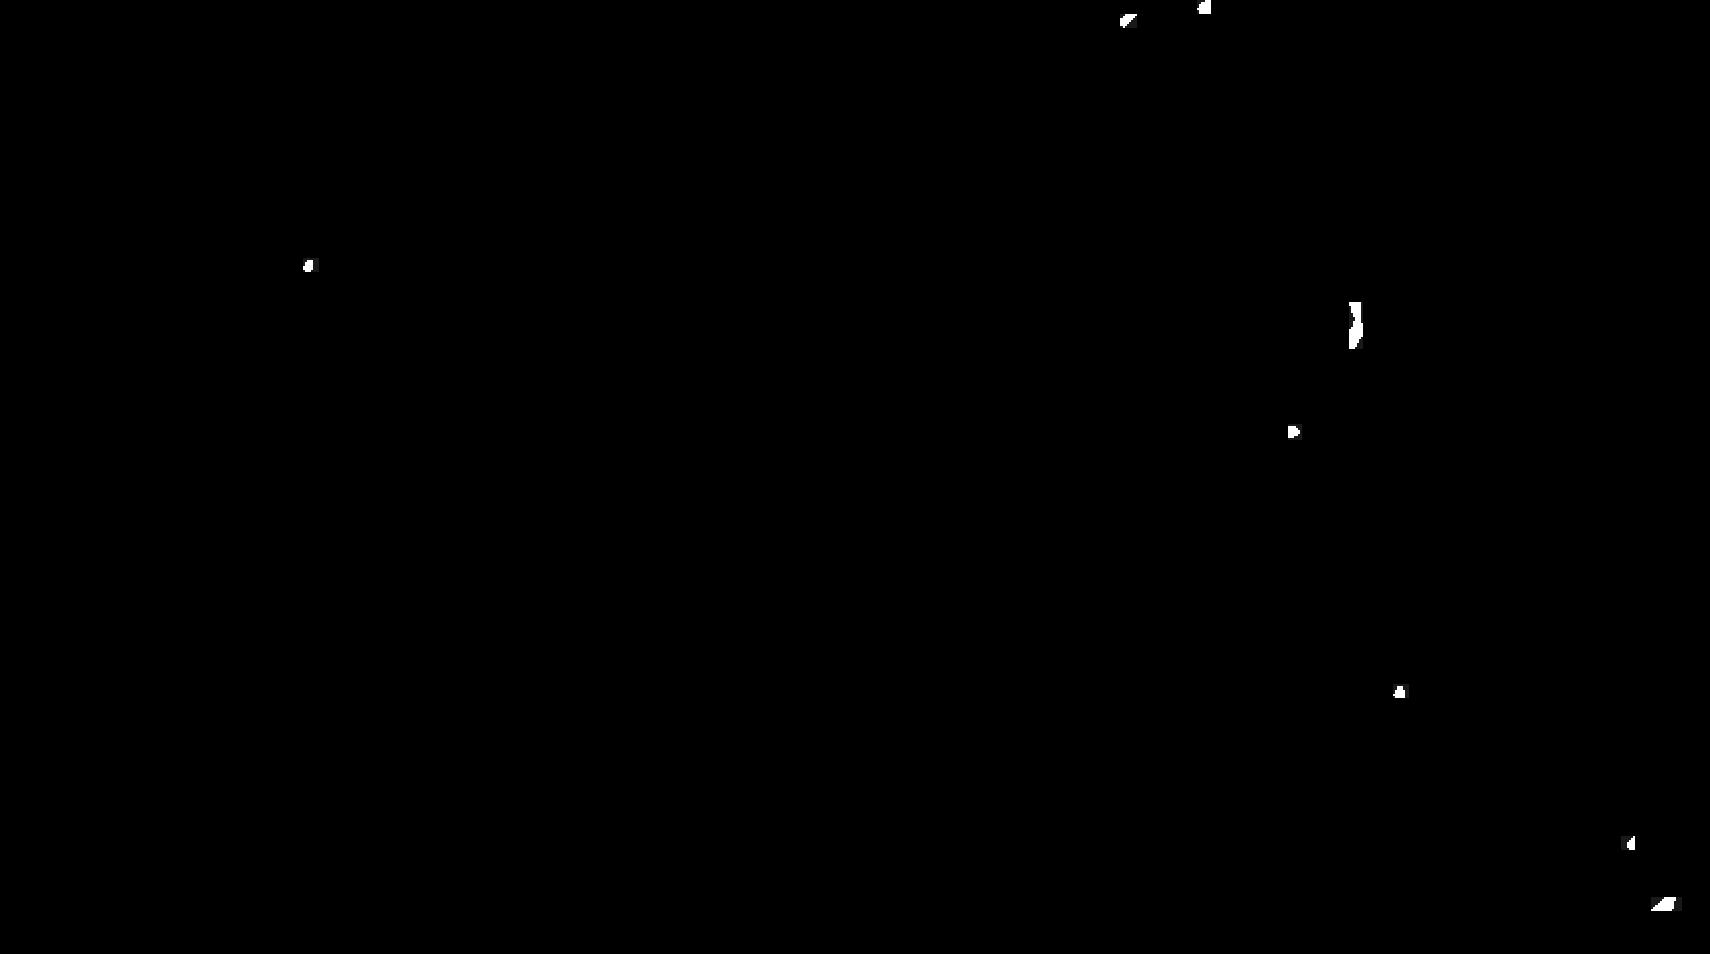
\includegraphics[width=.3\textwidth]{Imagenes/Homomorfico/Paranai1_masked_15.png}\hfill
    \\[\smallskipamount]
    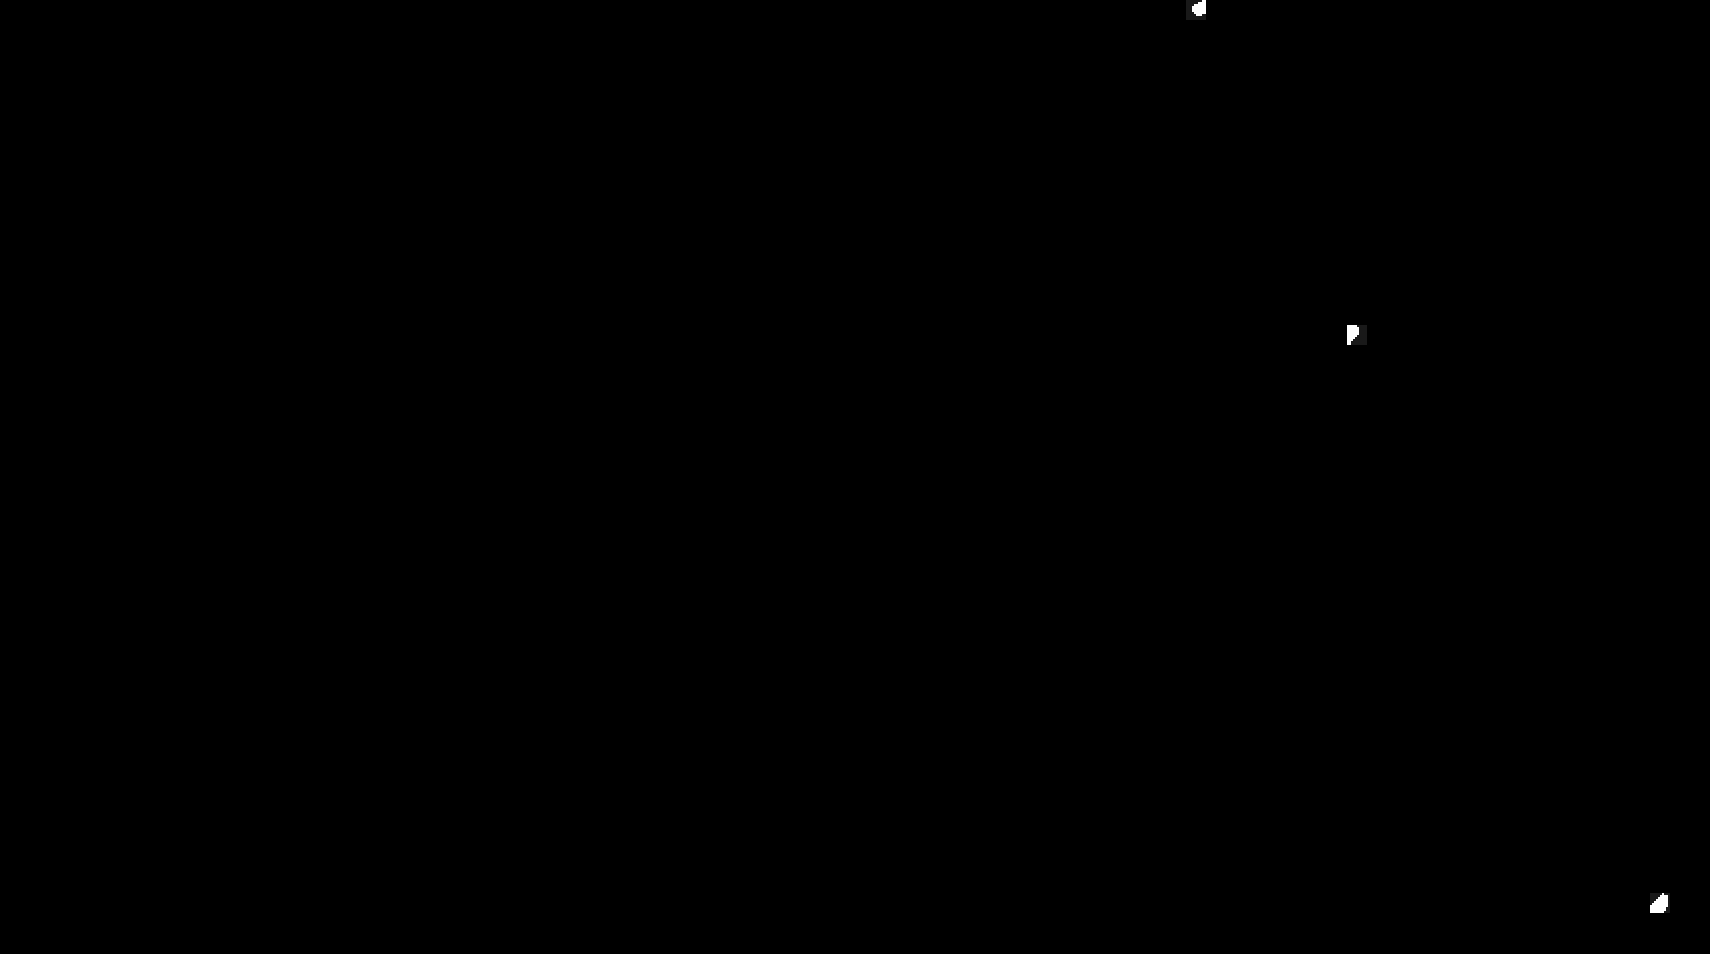
\includegraphics[width=.3\textwidth]{Imagenes/Homomorfico/Paranai1_masked_20.png}\hfill
    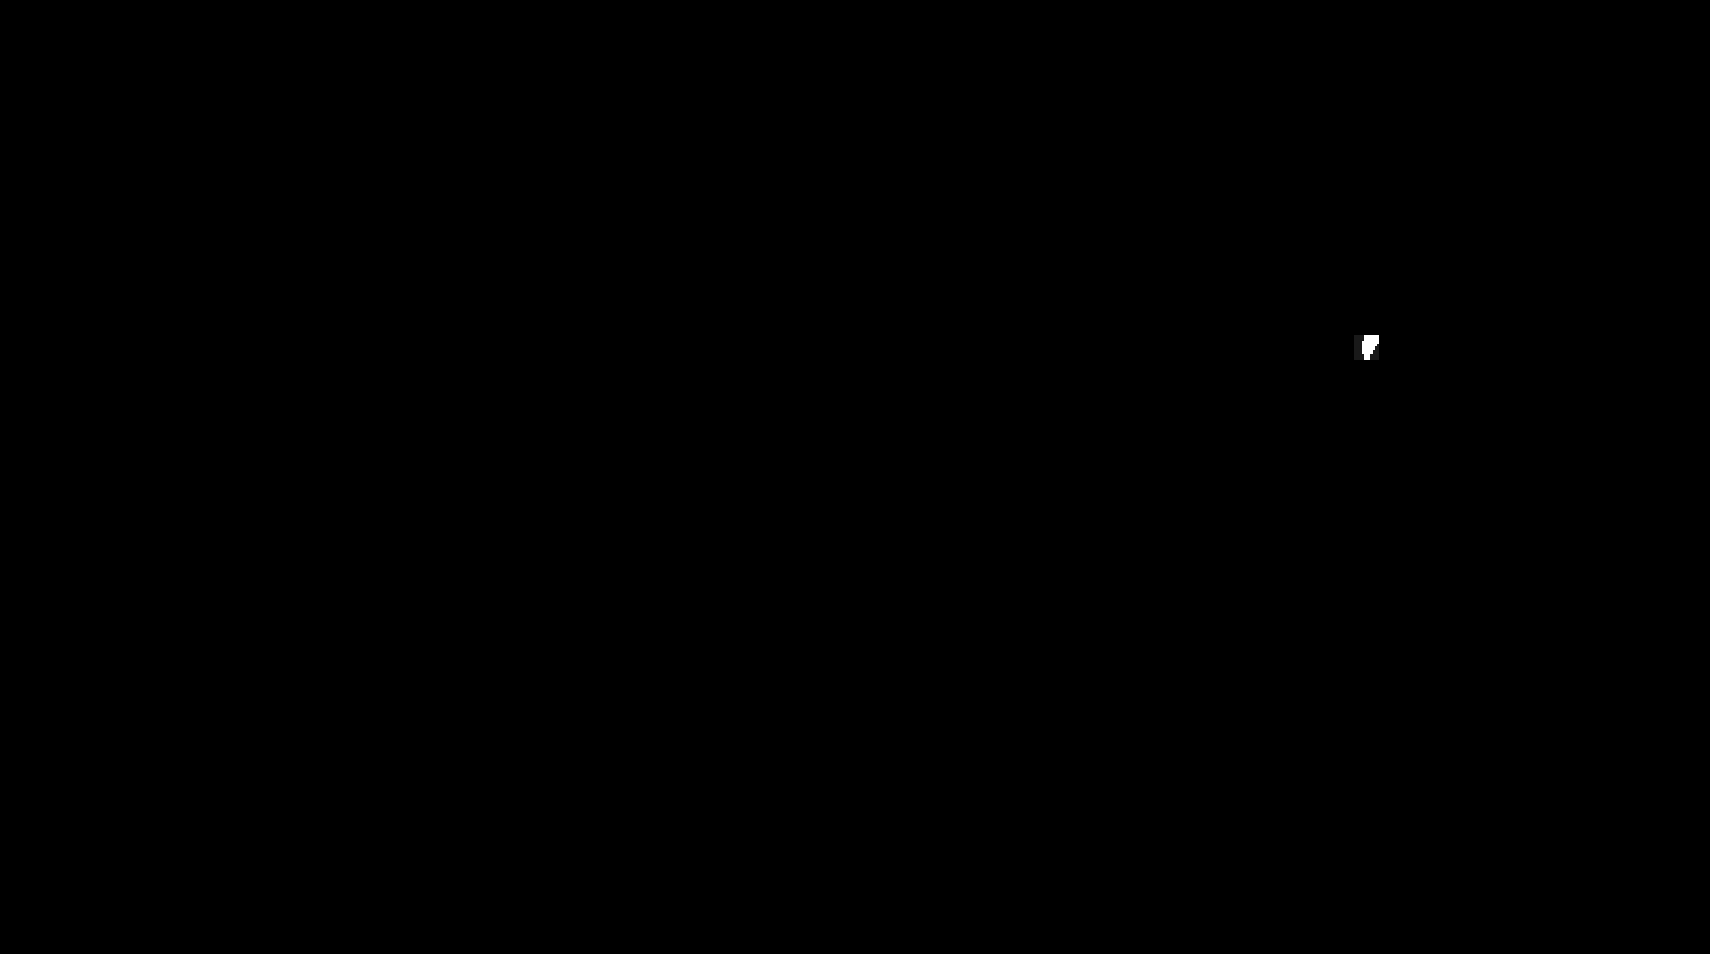
\includegraphics[width=.3\textwidth]{Imagenes/Homomorfico/Paranai1_masked_25.png}\hfill
    
\includegraphics[width=.3\textwidth]{Imagenes/Homomorfico/Paranai1_masked_30.png}\hfill
    
    \caption{Máscara binaria, sombras seleccionadas con ventana de 10, 15, 20, 25 y 30 píxeles}\label{fig:paranai1}
\end{figure}

\begin{figure}[h!]
    \includegraphics[width=0.5\textwidth]{Imagenes/Homomorfico/Paranai2eq.png}
     \hfill
     \caption{Imagen aérea (satelital) de una porción de selva nativa y terrenos cultivados junto al arroyo Paranay}
    %\label{Paranay2}
\end{figure}

\begin{figure}
    
\includegraphics[width=.3\textwidth]{Imagenes/Homomorfico/Paranai2_bin.png}\hfill
    
\includegraphics[width=.3\textwidth]{Imagenes/Homomorfico/Paranai2_masked_10.png}\hfill
    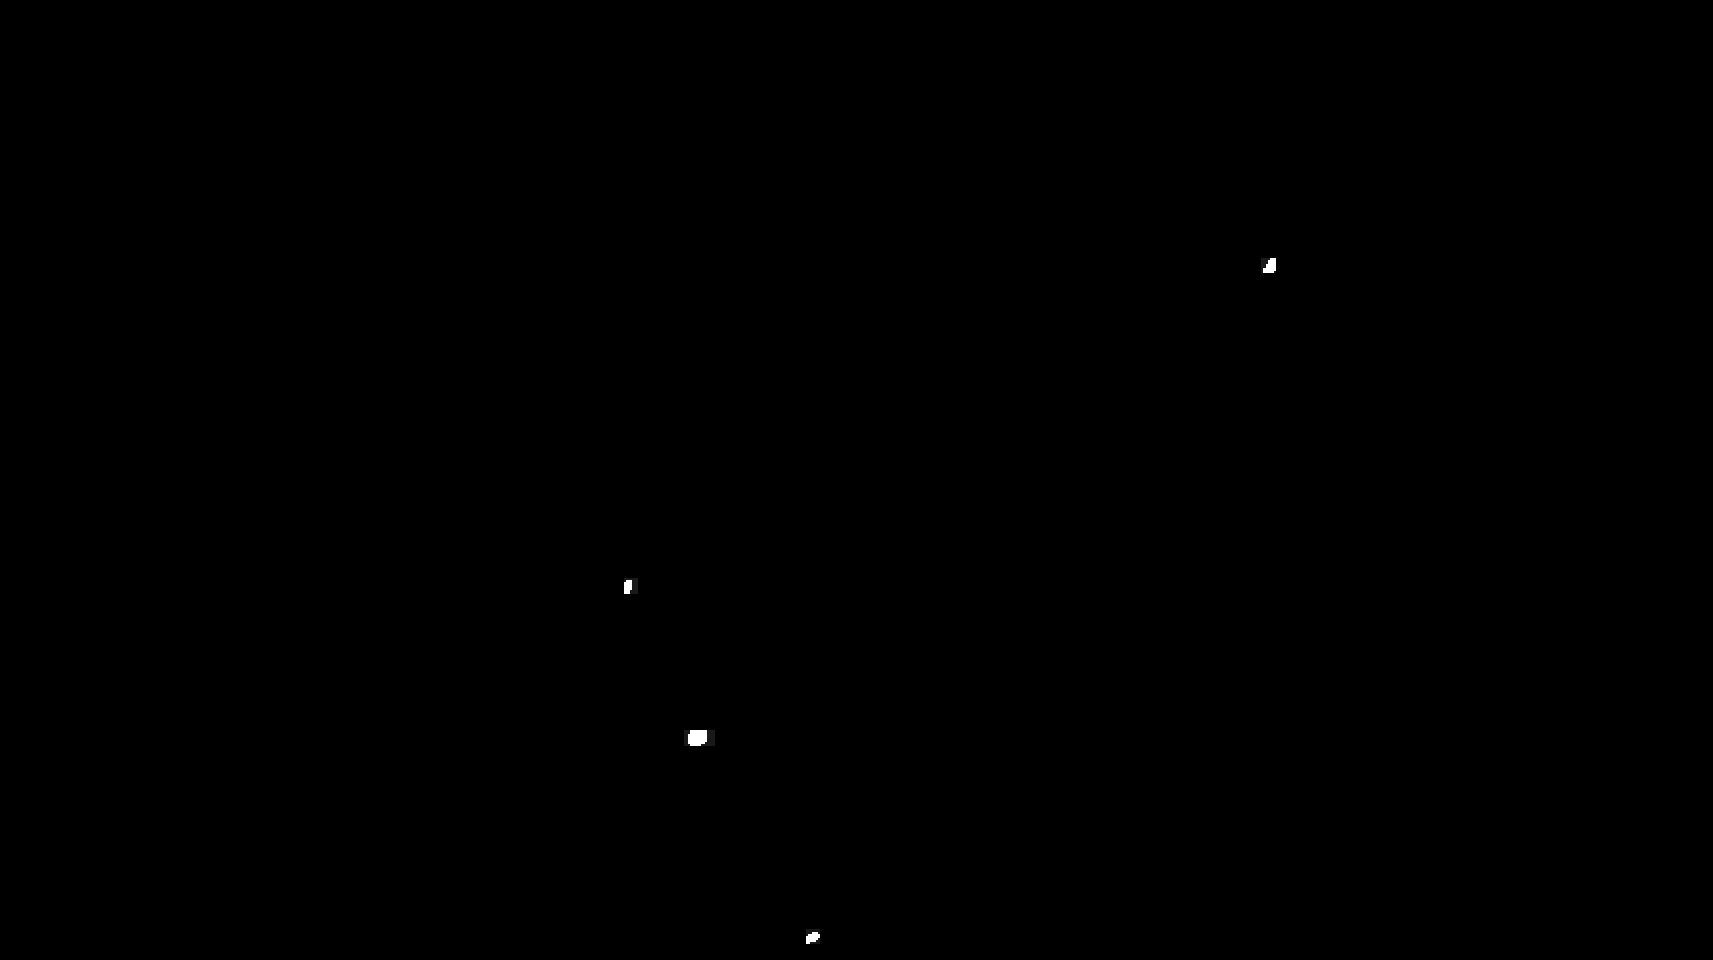
\includegraphics[width=.3\textwidth]{Imagenes/Homomorfico/Paranai2_masked_15.png}\hfill
    \\[\smallskipamount]
    
\includegraphics[width=.3\textwidth]{Imagenes/Homomorfico/Paranai2_masked_20.png}\hfill
    
\includegraphics[width=.3\textwidth]{Imagenes/Homomorfico/Paranai2_masked_25.png}\hfill
    
\includegraphics[width=.3\textwidth]{Imagenes/Homomorfico/Paranai2_masked_30.png}\hfill
    
    \caption{Máscara binaria, sombras seleccionadas con ventana de 10, 15, 20, 25 y 30 píxeles}\label{fig:Paranai2}
\end{figure}

\begin{figure}[h!]
    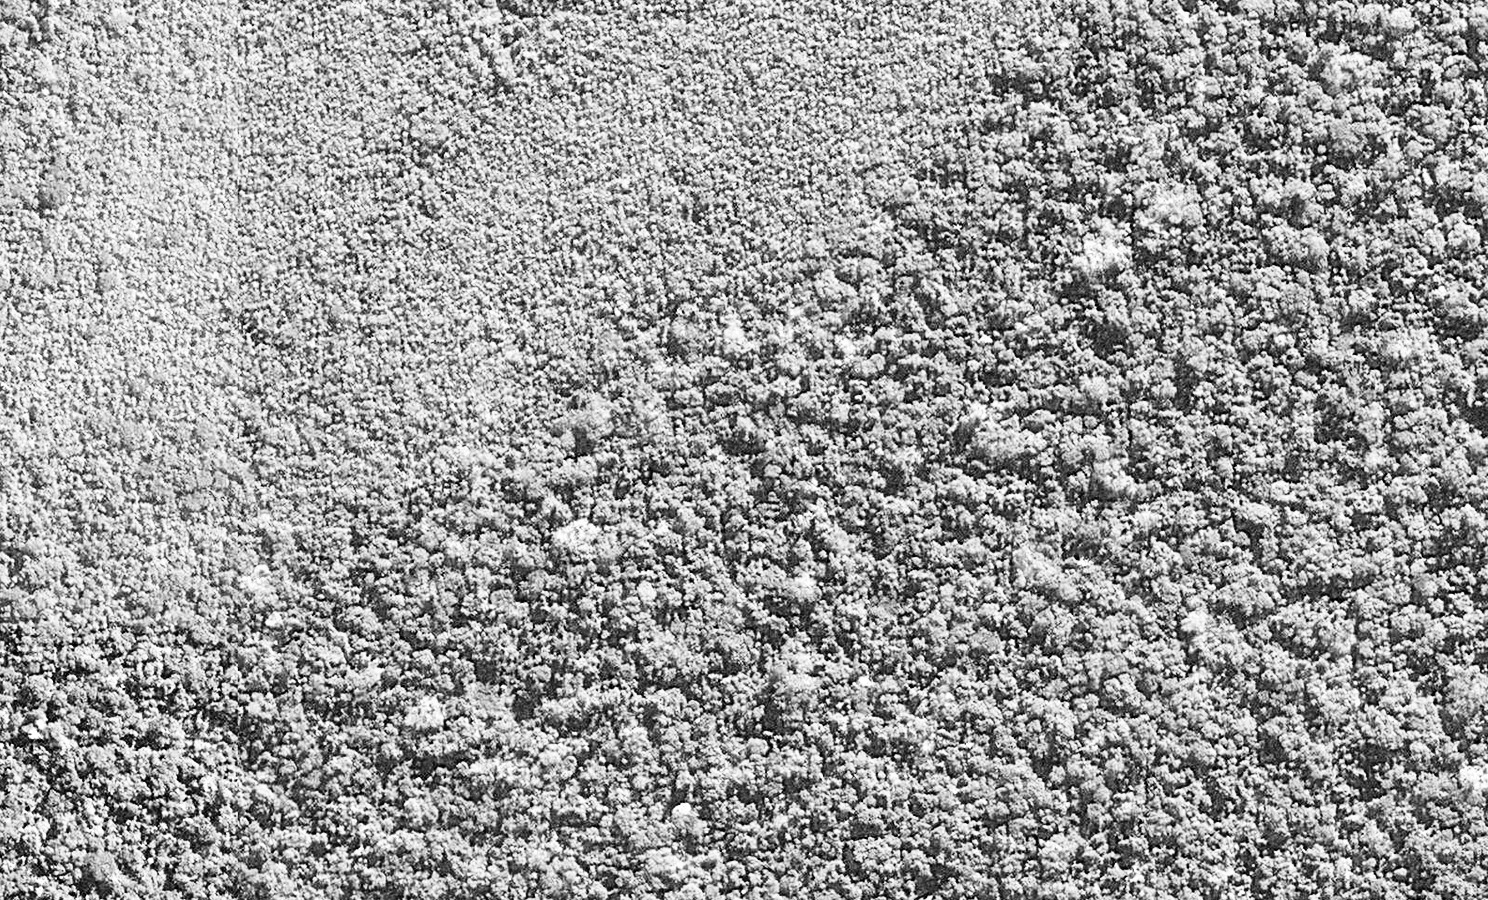
\includegraphics[width=0.5\textwidth]{Imagenes/Homomorfico/PNI1gris.jpg}
     \hfill
     \caption{Imagen aérea (satelital) Parque Nacional Iguazú, en escala de grises}
    %\label{PNI1}
\end{figure}

\begin{figure}[h!]
    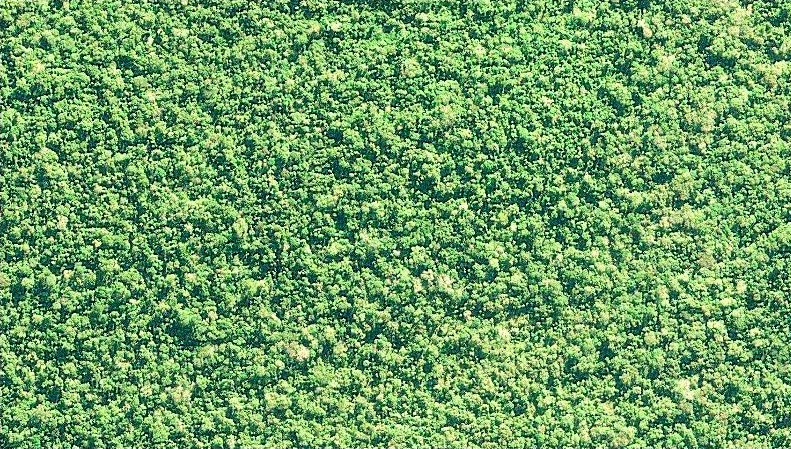
\includegraphics[width=0.5\textwidth]{Imagenes/Homomorfico/PNI2_original.jpg}
     \hfill
     \caption{Imagen aérea (satelital) Parque Nacional Iguazú, en RGB}
    %\label{PNI2}
\end{figure}

\begin{figure}
    
\includegraphics[width=.3\textwidth]{Imagenes/Homomorfico/PNI2_bin.png}\hfill
    
\includegraphics[width=.3\textwidth]{Imagenes/Homomorfico/PNI2_masked_10.png}\hfill
    
\includegraphics[width=.3\textwidth]{Imagenes/Homomorfico/PNI2_masked_15.png}\hfill
    \\[\smallskipamount]
    
\includegraphics[width=.3\textwidth]{Imagenes/Homomorfico/PNI2_masked_20.png}\hfill
    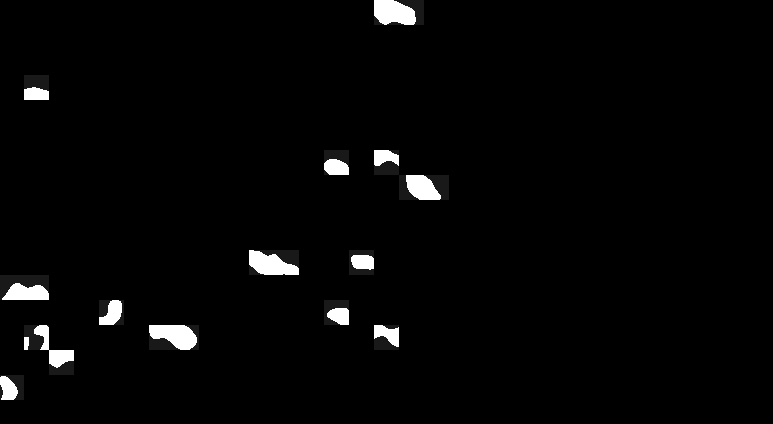
\includegraphics[width=.3\textwidth]{Imagenes/Homomorfico/PNI2_masked_25.png}\hfill
    
\includegraphics[width=.3\textwidth]{Imagenes/Homomorfico/PNI2_masked_30.png}\hfill
    
    \caption{Máscara binaria, sombras seleccionadas con ventana de 10, 15, 20, 25 y 30 píxeles}\label{fig:Iguazu2}
\end{figure}

\begin{figure}[h!]
    \includegraphics[width=0.5\textwidth]{Imagenes/Homomorfico/PNI_03.jpg}
     \hfill
     \caption{Imagen aérea (satelital) Parque Nacional Iguazú, en RGB}
    %  \label{PNI3}
\end{figure}

\begin{figure}[h!]
    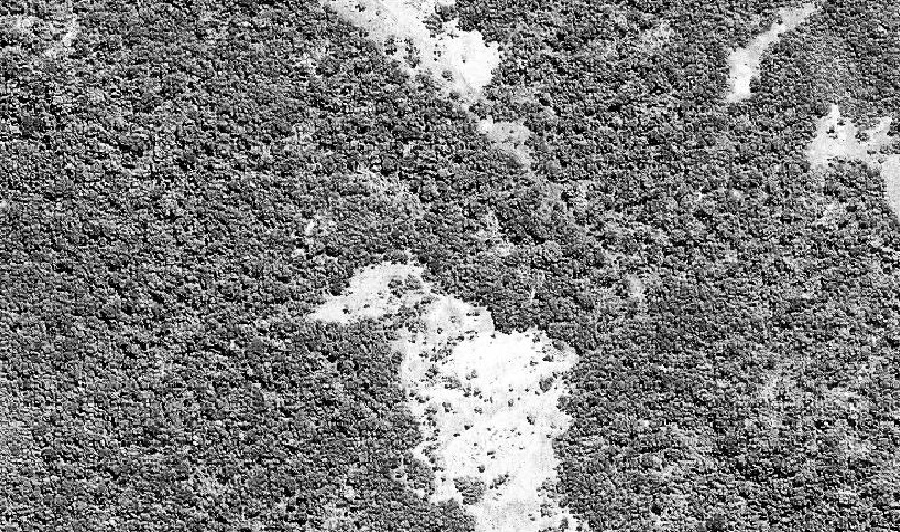
\includegraphics[width=0.5\textwidth]{Imagenes/Homomorfico/PS1_original.jpg}
     \hfill
     \caption{Imagen aérea (satelital) Parque de la Sierra, en RGB}
    %  \label{PS1}
\end{figure}

\begin{figure}
    
\includegraphics[width=.3\textwidth]{Imagenes/Homomorfico/PS1_bin.png}\hfill
    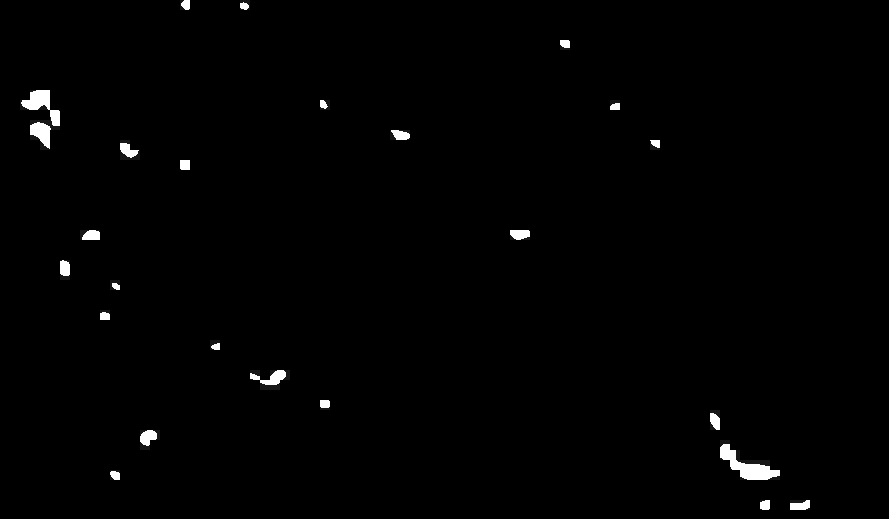
\includegraphics[width=.3\textwidth]{Imagenes/Homomorfico/PS1_masked_10.png}\hfill
    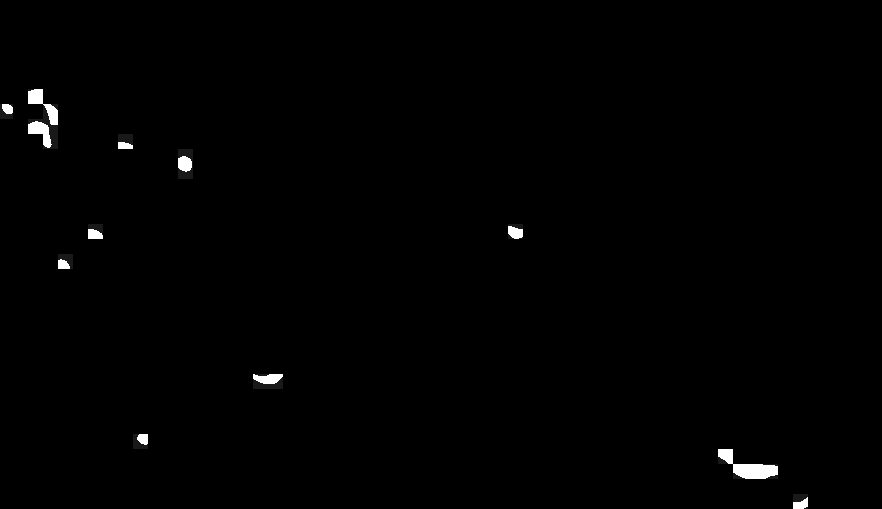
\includegraphics[width=.3\textwidth]{Imagenes/Homomorfico/PS1_masked_15.png}\hfill
    \\[\smallskipamount]
    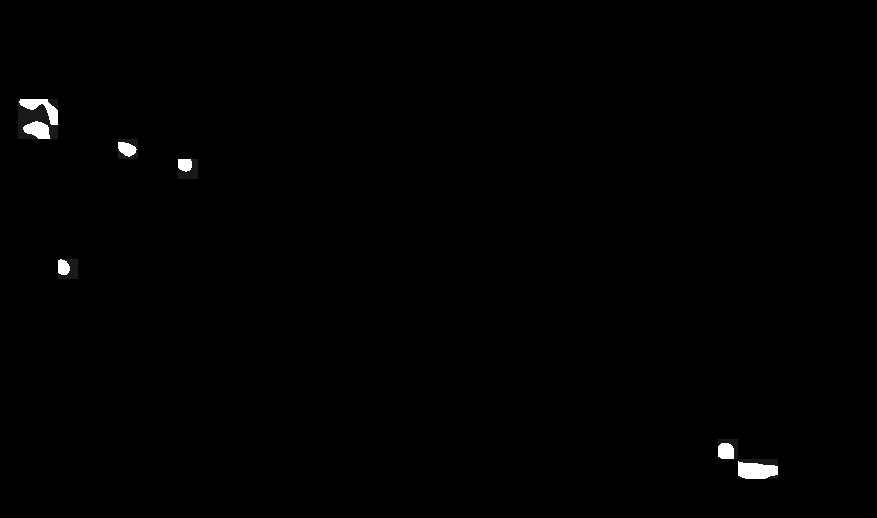
\includegraphics[width=.3\textwidth]{Imagenes/Homomorfico/PS1_masked_20.png}\hfill
    
\includegraphics[width=.3\textwidth]{Imagenes/Homomorfico/PS1_masked_25.png}\hfill
    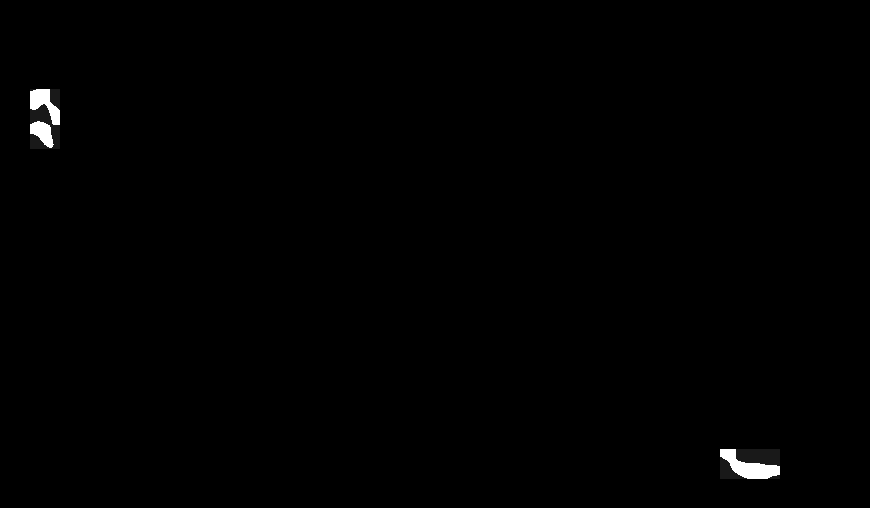
\includegraphics[width=.3\textwidth]{Imagenes/Homomorfico/PS1_masked_30.png}\hfill
    
    \caption{Máscara binaria, sombras seleccionadas con ventana de 10, 15, 20, 25 y 30 píxeles}\label{fig:Parque de la Sierra 1}
\end{figure}

\begin{figure}[h!]
    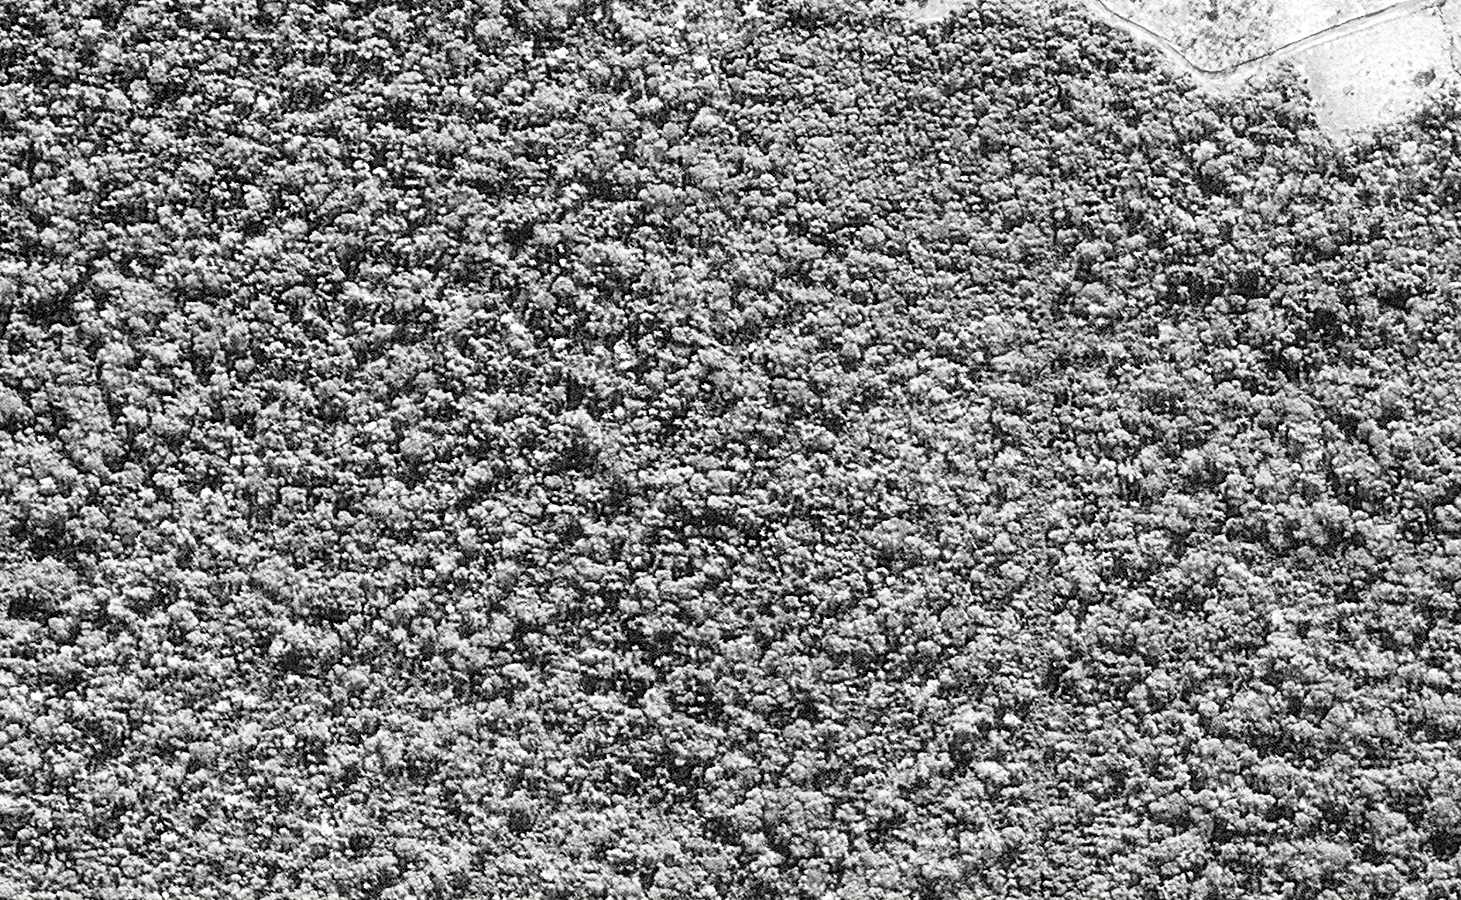
\includegraphics[width=0.5\textwidth]{Imagenes/Homomorfico/YB1.jpg}
     \hfill
     \caption{Imagen aérea (satelital) Biósfera Yaboty, en RGB}
    %  \label{YB1}
\end{figure}

\begin{figure}
    
\includegraphics[width=.3\textwidth]{Imagenes/Homomorfico/YB1_bin.png}\hfill
    
\includegraphics[width=.3\textwidth]{Imagenes/Homomorfico/YB1_masked_10.png}\hfill
    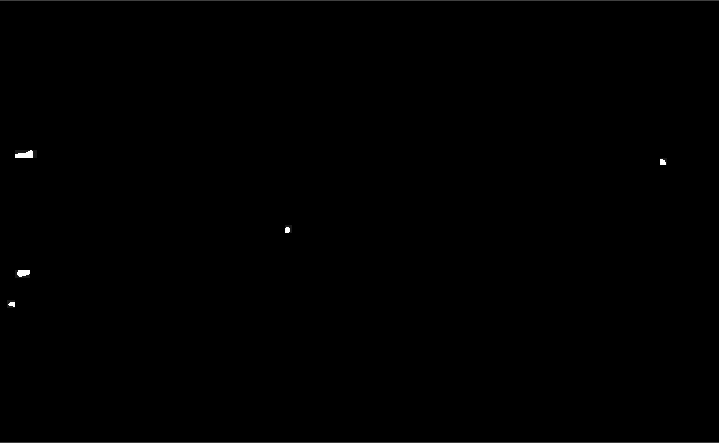
\includegraphics[width=.3\textwidth]{Imagenes/Homomorfico/YB1_masked_15.png}\hfill
    \\[\smallskipamount]
    
\includegraphics[width=.3\textwidth]{Imagenes/Homomorfico/YB1_masked_20.png}\hfill
    
\includegraphics[width=.3\textwidth]{Imagenes/Homomorfico/YB1_masked_25.png}\hfill
    
\includegraphics[width=.3\textwidth]{Imagenes/Homomorfico/YB1_masked_30.png}\hfill
    
    \caption{Máscara binaria, sombras seleccionadas con ventana de 10, 15, 20, 25 y 30 píxeles}\label{fig:Yaboty1}
\end{figure}

\begin{figure}[h!]
    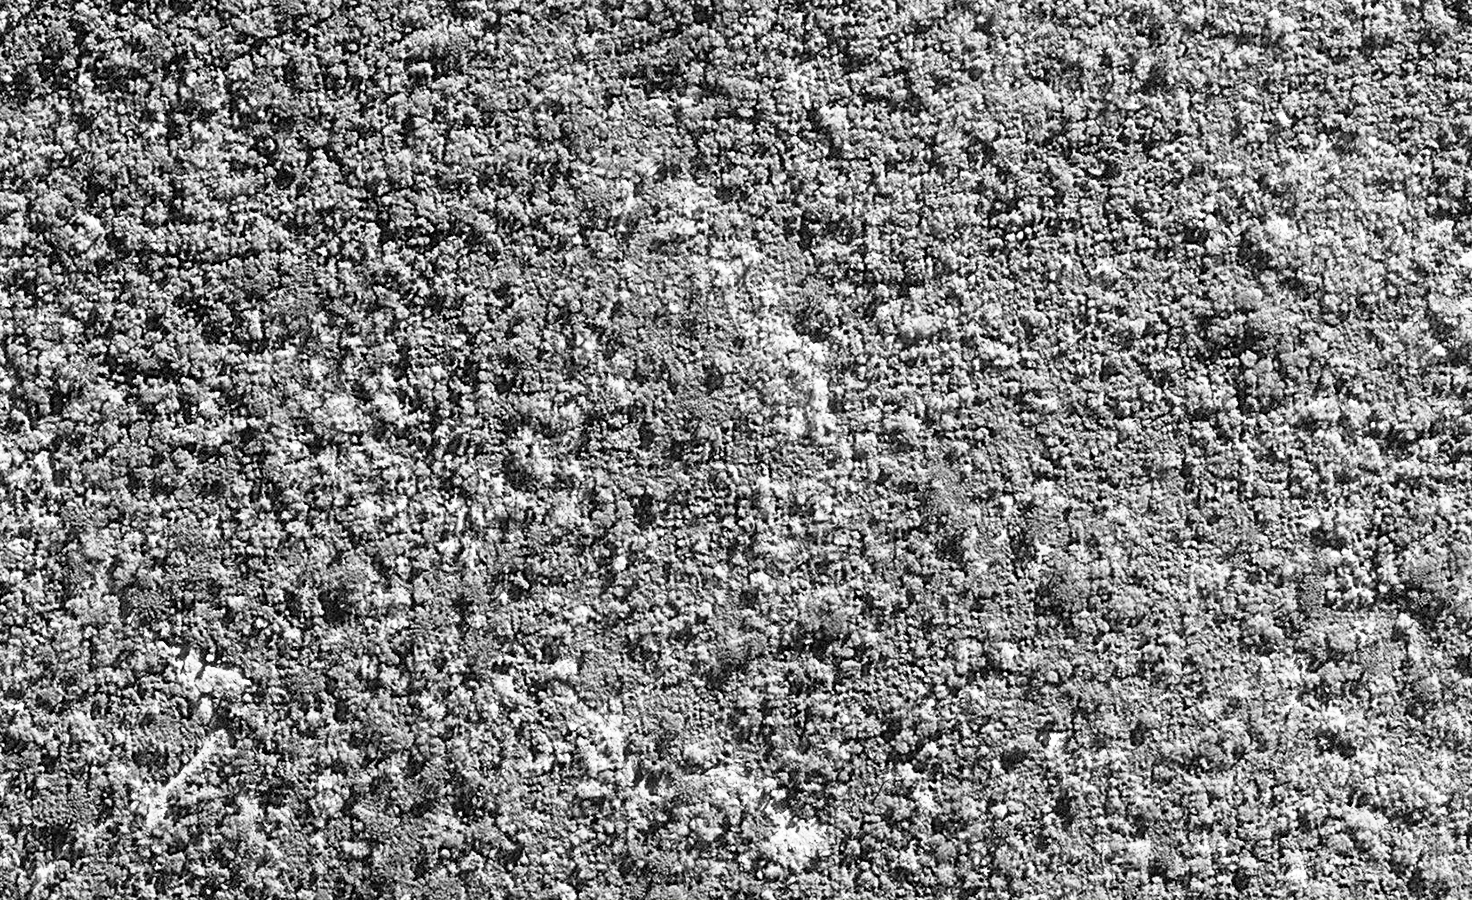
\includegraphics[width=0.5\textwidth]{Imagenes/Homomorfico/YB2.jpg}
     \hfill
     \caption{Imagen aérea (satelital) Biósfera Yaboty, en RGB}
    %  \label{YB2}
\end{figure}

\begin{figure}
    
\includegraphics[width=.3\textwidth]{Imagenes/Homomorfico/YB2_bin.png}\hfill
    
\includegraphics[width=.3\textwidth]{Imagenes/Homomorfico/YB2_masked_10.png}\hfill
    
\includegraphics[width=.3\textwidth]{Imagenes/Homomorfico/YB2_masked_15.png}\hfill
    \\[\smallskipamount]
    
\includegraphics[width=.3\textwidth]{Imagenes/Homomorfico/YB2_masked_20.png}\hfill
    
\includegraphics[width=.3\textwidth]{Imagenes/Homomorfico/YB2_masked_25.png}\hfill
    
\includegraphics[width=.3\textwidth]{Imagenes/Homomorfico/YB2_masked_30.png}\hfill
    
    \caption{Máscara binaria, sombras seleccionadas con ventana de 10, 15, 20, 25 y 30 píxeles}\label{fig:Yaboty2}
\end{figure}

\begin{figure}[h!]
    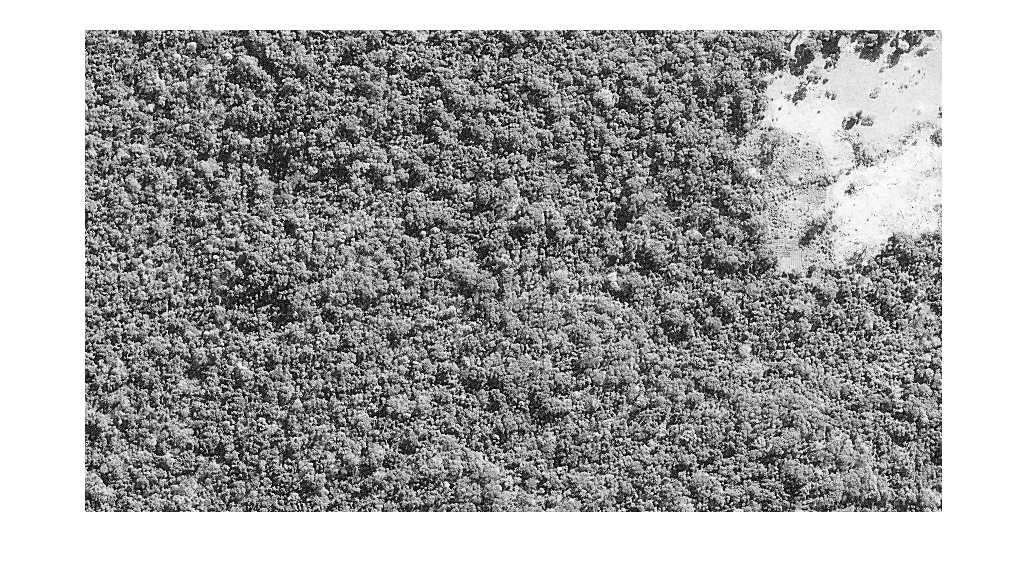
\includegraphics[width=0.5\textwidth]{Imagenes/Homomorfico/ST1_gris.png}
     \hfill
     \caption{Imagen aérea (satelital) reserva privada Sombra de Toro, en escala de grises}
    %  \label{ST1}
\end{figure}

\begin{figure}
    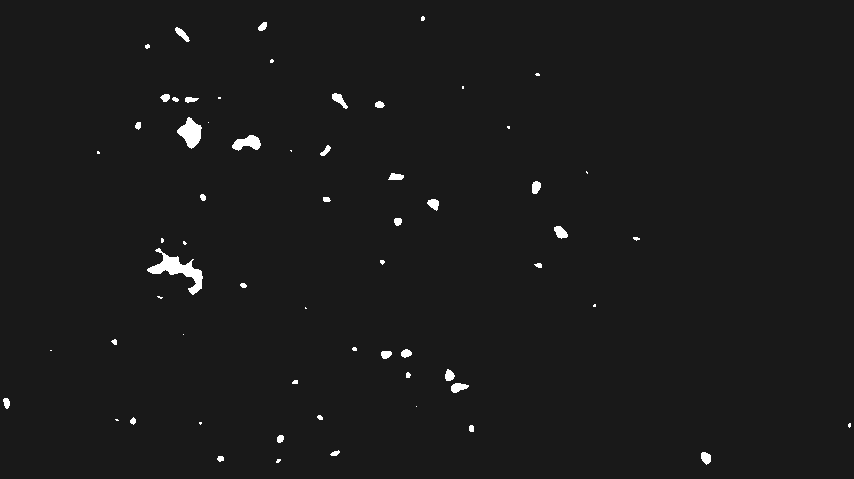
\includegraphics[width=.3\textwidth]{Imagenes/Homomorfico/ST1_bin.png}\hfill
    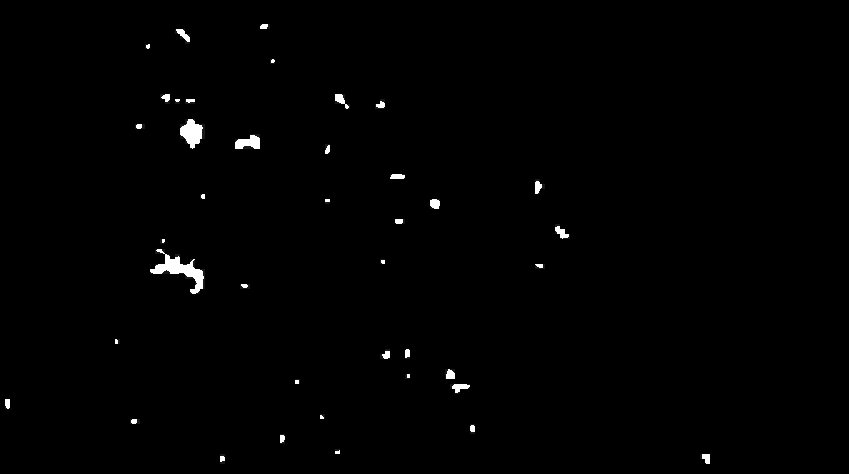
\includegraphics[width=.3\textwidth]{Imagenes/Homomorfico/ST1_masked_10.png}\hfill
    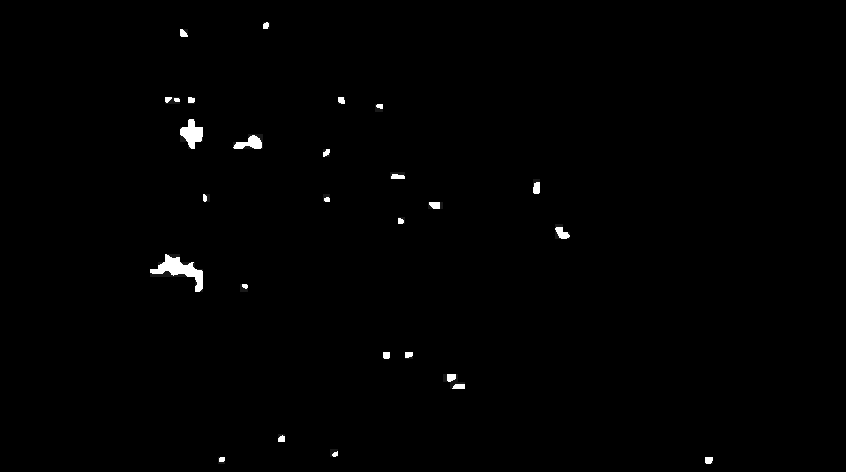
\includegraphics[width=.3\textwidth]{Imagenes/Homomorfico/ST1_masked_15.png}\hfill
    \\[\smallskipamount]
    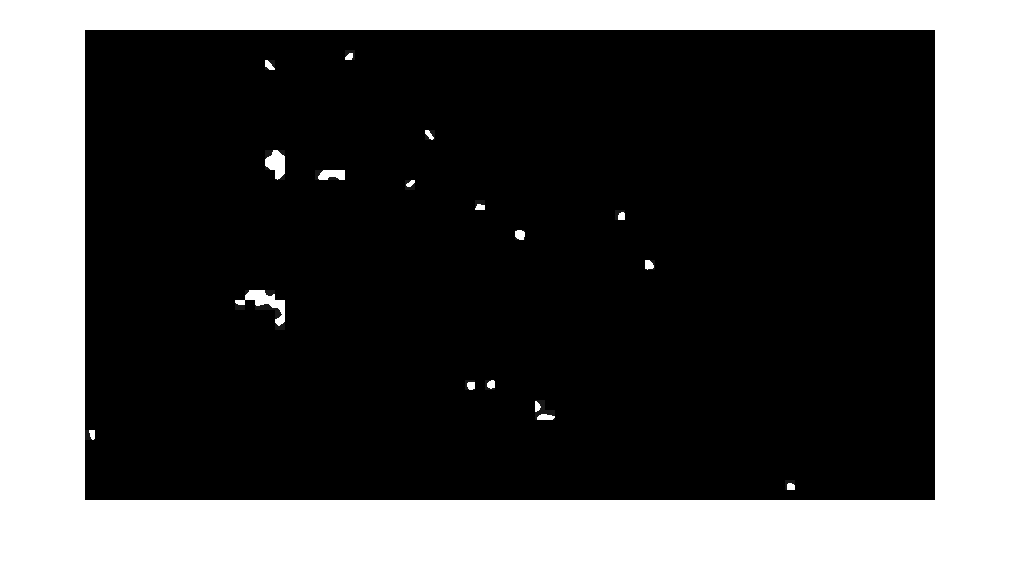
\includegraphics[width=.3\textwidth]{Imagenes/Homomorfico/ST1_masked_20.png}\hfill
    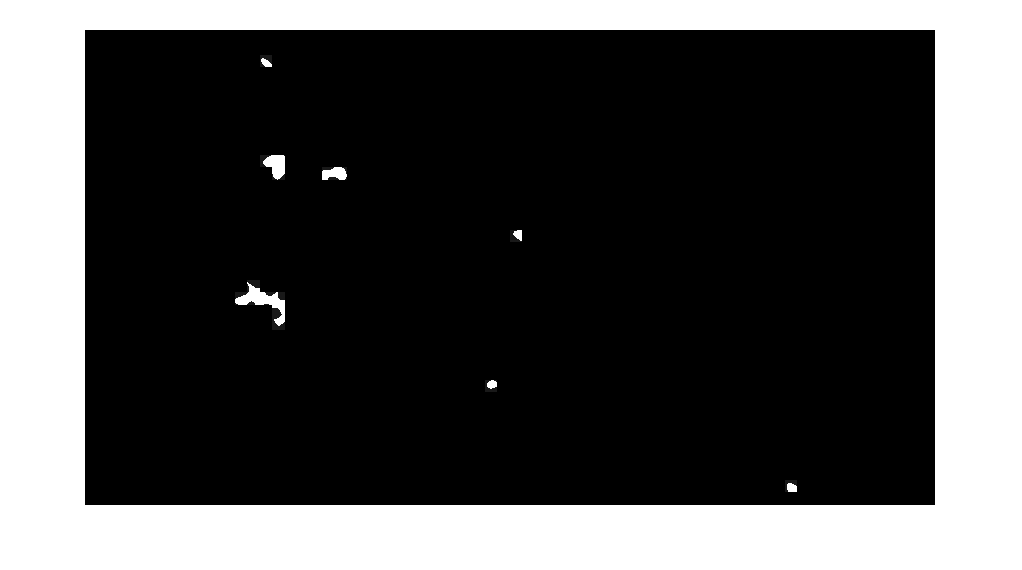
\includegraphics[width=.3\textwidth]{Imagenes/Homomorfico/ST1_masked_25.png}\hfill
    \includegraphics[width=.3\textwidth]{Imagenes/Homomorfico/ST1_masked_30.png}\hfill
    
    \caption{Máscara binaria, sombras seleccionadas con ventana de 10, 15, 20, 25 y 30 píxeles}\label{fig:Storo1}
\end{figure}

\begin{figure}[h!]
    \includegraphics[width=0.5\textwidth]{Imagenes/Homomorfico/ST2.png}
     \hfill
     \caption{Imagen aérea (satelital) reserva privada Sombra de Toro, en RGB}
    %  \label{ST2}
\end{figure}

\begin{figure}
    \includegraphics[width=.3\textwidth]{Imagenes/Homomorfico/ST2_bin.png}\hfill
    \includegraphics[width=.3\textwidth]{Imagenes/Homomorfico/ST2_masked_10.png}\hfill
    \includegraphics[width=.3\textwidth]{Imagenes/Homomorfico/ST2_masked_15.png}\hfill
    \\[\smallskipamount]
    \includegraphics[width=.3\textwidth]{Imagenes/Homomorfico/ST2_masked_20.png}\hfill
    \includegraphics[width=.3\textwidth]{Imagenes/Homomorfico/ST2_masked_25.png}\hfill
    \includegraphics[width=.3\textwidth]{Imagenes/Homomorfico/ST2_masked_30.png}\hfill
    
    \caption{Máscara binaria, sombras seleccionadas con ventana de 10, 15, 20, 25 y 30 píxeles}\label{fig:Storo2}
\end{figure}

